\documentclass{beamer}

\usepackage[utf8]{inputenc}
\usepackage{graphicx}
\graphicspath{ {./Figures/} }

\title{Modeling Price and Popularity of AirBnB listings in New-York}
\author{Melody Jiang, Raphael Morsomme, Ezinne Nwankwo}
\institute{Department of Statistical Science, Duke University}
\date{02/03/2020}

\begin{document}

\frame{\titlepage}



%%%%%%%%%% Section1: Introduction %%%%%%%%%%%


\begin{frame}
\frametitle{Overview}

\begin{itemize}
\item Data: Airbnblistings in NYC from 2019, 48,895 listings, 16 variables

\item Questions
\begin{itemize}
    \item Influential factors on popularity / price
    \item Heterogeneity among boroughs
    \item If the type of listing vary across neighbourhoods
    \item Where to locate listing and how to name listing to make listing most expensive and popular
\end{itemize}


\end{itemize}

\end{frame}

\begin{frame}
    \frametitle{EDA - Issues with data}
    \begin{itemize}
        \item Constructing a measure of popularity from limiting variables (time of last review)
        \item Improbable values
        \item ideally , tidy data (Wickham, 2009) with one row per booking
        \item Focus on data cleanin g and feature en g ineering over modeling.
        \item EDA will motivate the creation of new variables and the cleaning of the data.
    \end{itemize}
\end{frame}

\begin{frame}
    \frametitle{EDA - A city of two tales}

    
    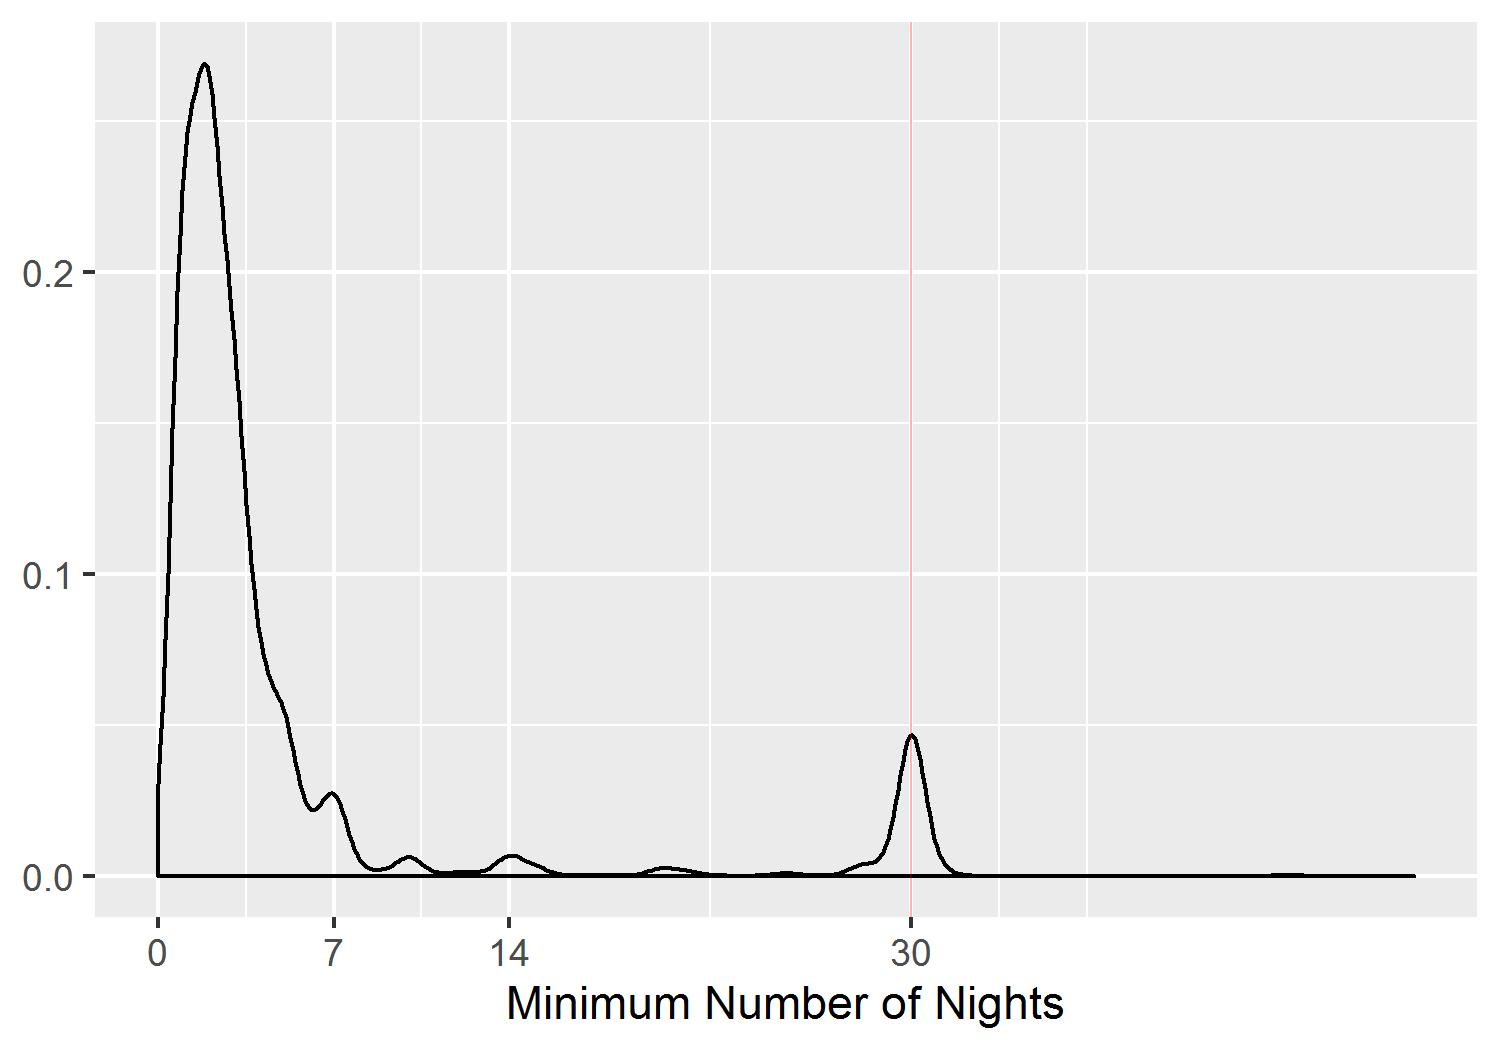
\includegraphics[scale = 0.8]{length_stay_density.jpeg}
\end{frame}

\begin{frame}
    \frametitle{EDA - Are you available?}

    
\end{frame}

\begin{frame}
    \frametitle{EDA - Attractions}
    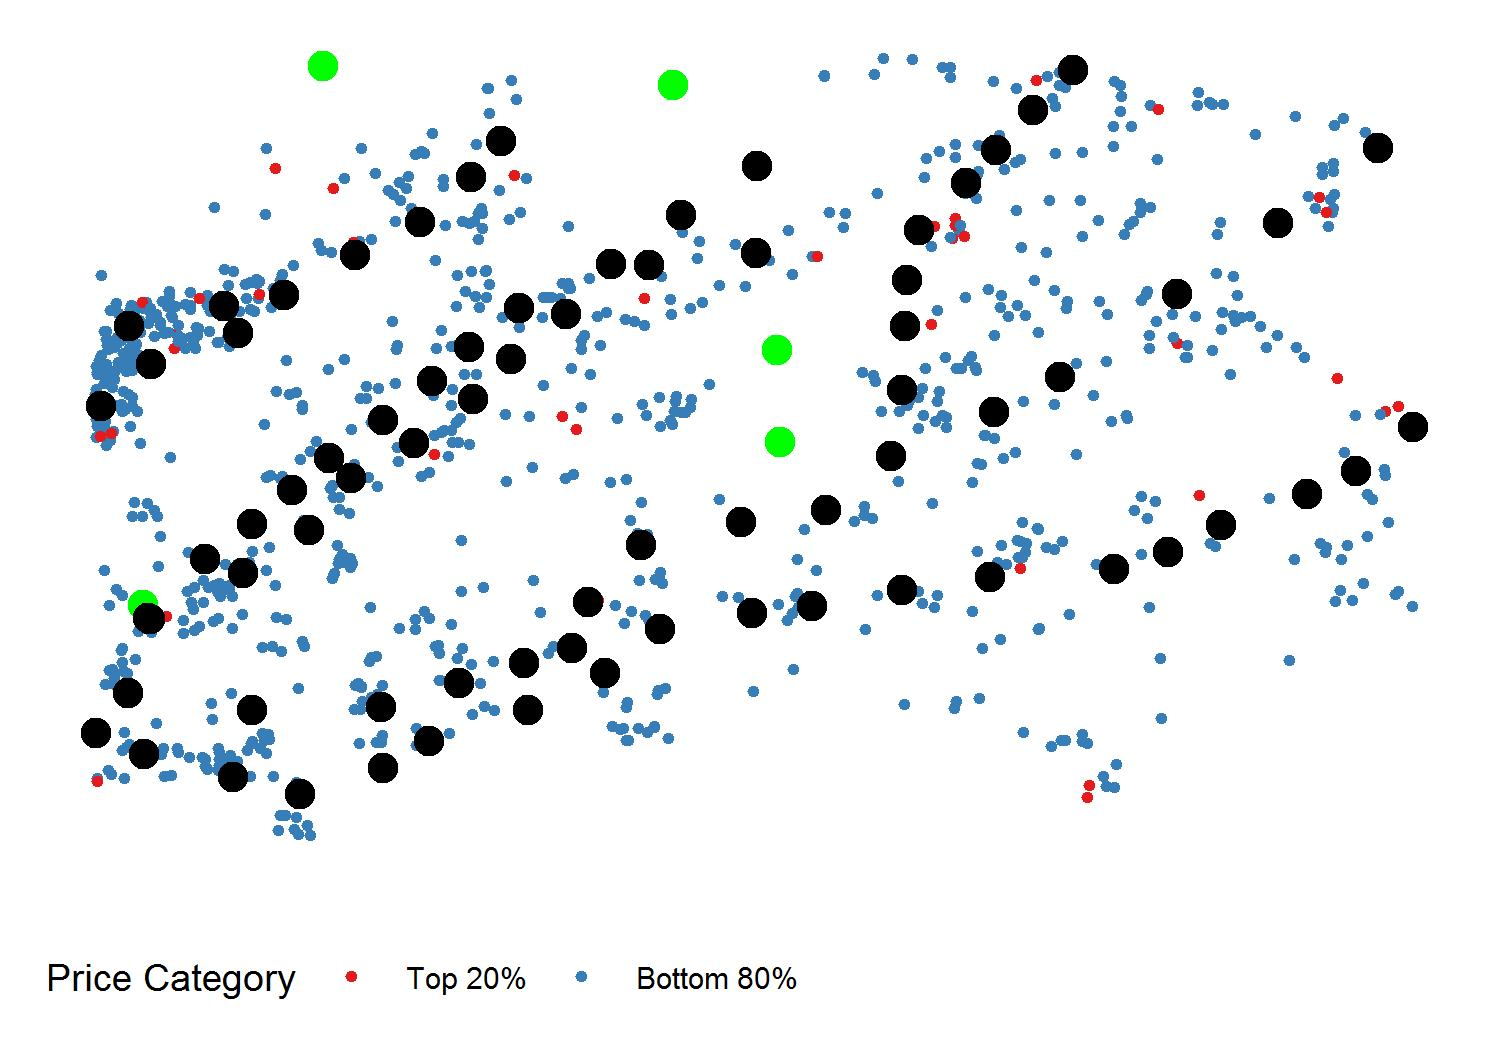
\includegraphics[scale = 0.8]{map_eda.jpeg}
\end{frame}

\begin{frame}
    \frametitle{EDA - Attractions}
    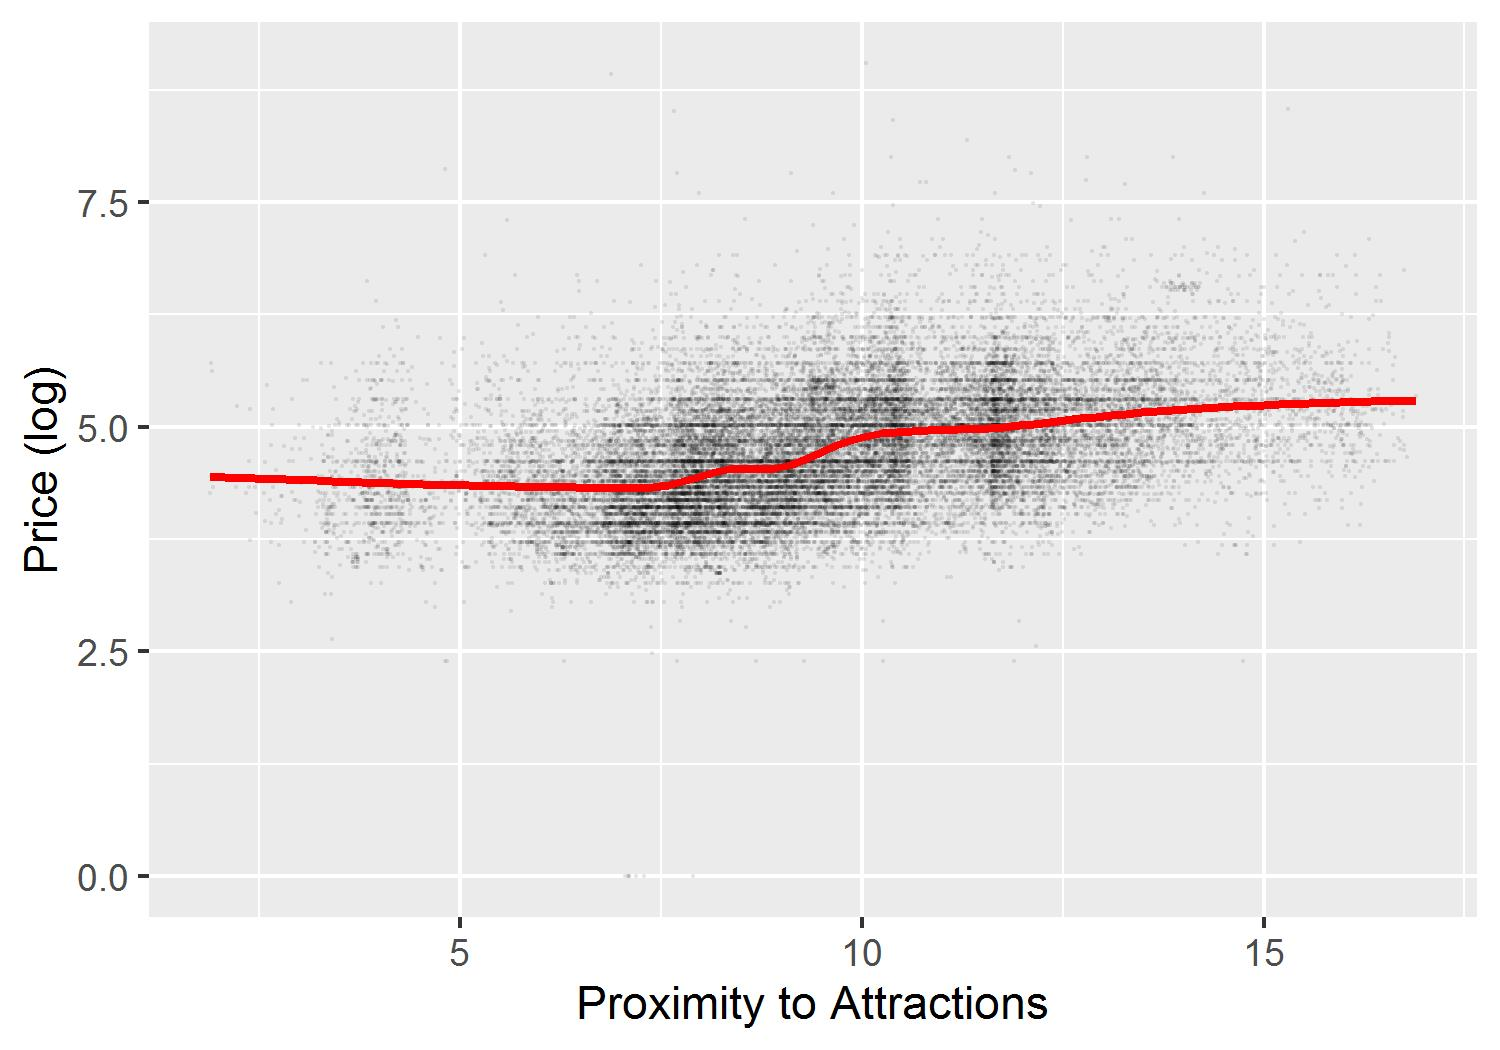
\includegraphics[scale = 0.8]{log_price_vs_prox_attr.jpeg}
\end{frame}

\begin{frame}
    \frametitle{EDA - Metro}
    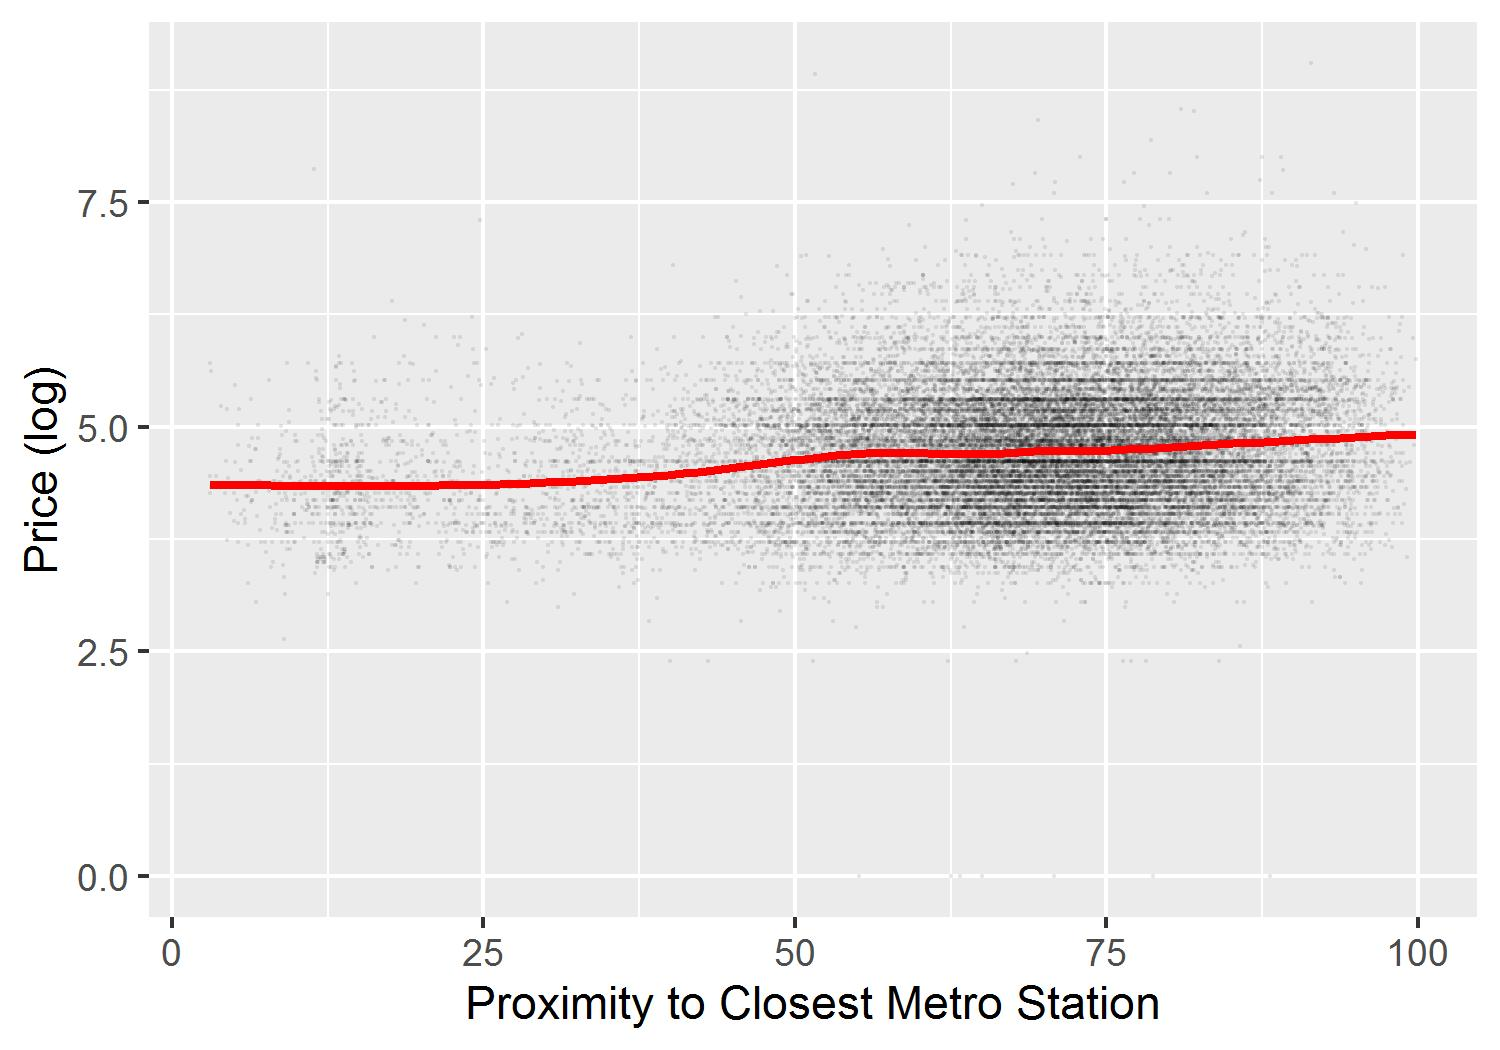
\includegraphics[scale = 0.8]{log_price_vs_prox_metro.jpeg}
\end{frame}

\section{Data Cleaning}


\begin{frame}
    \frametitle{Data Cleaning}
    Drawing on the EDA, focus on \underline{active} listings for \underline{short stay}:
    
    Keep listings with
    
    (i) last review < 1 year old [lose $15,000$]
    
    (ii) minimum number days $< 30$ (short type of stay) [lose $XXX$]
    
\end{frame}

\begin{frame}

    \frametitle{Data Cleaning}
    \begin{itemize}
        \item Days since last review
        \begin{itemize}
            \item not indicative of price nor popularity
            \item A rough indicator of activeness of listing
        \end{itemize}
        \item Calculated host listings
        \begin{itemize}
            \item Exclude listings whose calculated host listings $>5$
            \item Different type of business
        \end{itemize}
        \item Number of available days in a year
        \begin{itemize}
            \item Excluded this variable, as we used it to calculate popularity
        \end{itemize}
    \end{itemize}

\end{frame}

\section{Feature Engineering}
\begin{frame}{Feature Engineering - Proximity}
EDA shows impact of attraction on price. This suggests the creation of a variable measuring the proximity of a listing to attractions. The proximity variable is defined as the average proximity of the listing to the attractions
$$proximity(X) = \dfrac{1}{n}\sum_{i=1}^{n} \dfrac{1}{dist(X, attraction_i)}
$$
where
$$ 
dist(x, y) = \mid latitude_{x} - latitutde_{y} \mid +  \mid longitude_{x} - longitude_{y} \mid.
$$
is the Manhattan distance.

Similarly, we compute the proximity to the closest metro station.
\end{frame}

\begin{frame}{Feature Engineering - Textual Data}

Sentiment analysis of listing name

- "documents" too short for topic modeling
- Afinn dictionary (gradual rating)

$$ Sentiment(X) = \dfrac{1}{n}\sum_{i=1}^{n} dictionary(x_i)
$$
where $Afinn(x) \in \left\lbrace -5, -4, \dots, 5\right\rbrace $.

Origin of host name 

- use name frequency as a proxy

\end{frame}

\section{Models}
\begin{frame}{Models}
Linear regression model $Y = X \beta$
where $X$ consists of:

proximity metro, proximity attraction, host name frequency, listing name sentiment, [newly created variables]

X1, X2, X3 [regular variable]

Random forest (n = $1,500$, m = $2/3$)

BMA (setting)
\end{frame}

\begin{frame}{Influential Factors}
\textit{Variable Importance} metric from the random forest (n = $1,500$, m = $2/3$)

\textit{Posterior Inclusion Probability} from the BMA
\end{frame}

\begin{frame}{Sensitivity Analysis}
Vary the setting of the RF: different levels of pruning, different values for $m$.

Vary the priors in the BMA: prior1, prior2, prior3
\end{frame}


%%%%%%%
\section{Results}
\begin{frame}{Results - Influential Factors}
<Table of variable importance>

<Table of PIP>
\end{frame}

\begin{frame}{Results - Q3}
<Figure for Q3>
\end{frame}

%%%%%%%
\begin{frame}
    \frametitle{Discussions}

    \begin{itemize}
        \item Incusion of boroughs does not work well. Spatial modeling that addresses relationship between houses.(http://citeseerx.ist.psu.edu/viewdoc/download?doi=10.1.1.532.451&rep=rep1&type=pdf)
        \item Submarkets influence pricing. Finite mixture model. (https://pages.jh.edu/jrer/papers/pdf/forth/accepted/using%20a%20finite%20mixture%20model%20of%20heterogeneous%20households%20to%20delineate%20housing%20submarkets.pdf)
    \end{itemize}

\end{frame}



\begin{frame}
\frametitle{References}
\footnotesize{
	\begin{thebibliography}{99} % Beamer does not support BibTeX so references must be inserted manually as below
		
		\bibitem[Whickam, 2013]{Whickam2009} Whickam, H. \\
		\newblock Tidy Data\\
		\newblock \emph{Journal}, month year
		
	\end{thebibliography}
}
\end{frame}
    






\end{document}
